\documentclass[a4paper, 12pt]{article}

\usepackage[utf8]{inputenc}
\usepackage[T1]{fontenc}
\usepackage[french]{babel}
%\usepackage{layout}
\usepackage[top=3cm, bottom=3cm, left=2.5cm, right=2.5cm]{geometry}\usepackage{setspace} %interligne
%\usepackage{soul}
%\usepackage{ulem}
%\usepackage{eurosym}
%\usepackage{bookman}
%\usepackage{charter}
%\usepackage{newcent}
%\usepackage{lmodern}
%\usepackage{mathpazo}
%\usepackage{mathptmx}
%\usepackage{url}
\usepackage{graphicx}
\usepackage{verbatim}
%\usepackage{moreverb}
%\usepackage{listings}
\usepackage{fancyhdr}
%\usepackage{wrapfig}
%\usepackage{color}
%\usepackage{colortbl}
\usepackage{amsmath}
\usepackage{amssymb}
\usepackage{mathrsfs}
%\usepackage{asmthm}
%\usepackage{makeidx}
\usepackage{lastpage}
\usepackage{float}

\usepackage{listings}
\lstset{
language=VHDL,
basicstyle=\footnotesize,
numberstyle=\normalsize,
numbersep=7pt,
}

\pagestyle{fancy}

\renewcommand\headrulewidth{1pt}
\fancyhead[L]{Alexandre LADRIERE - EI17}
\fancyhead[R]{VHDL: Algorithme de déchiffrement AES 128bits}
\renewcommand\footrulewidth{1pt}
\fancyfoot[C]{
\textbf{Page \thepage/\pageref{LastPage}}}

\onehalfspacing

\title{\huge{\begin{bf} Programmation et conception de systèmes numériques\end{bf}} \\ \begin{doublespacing} \large{Modélisation VHDL de l'algorithme de déchiffrement AES 128bits} \end{doublespacing} \vspace{\fill}}
\author{Alexandre LADRIERE}
\date{9 Décembre 2018}

\begin{document}

	\begin{figure}
	\begin{center}
	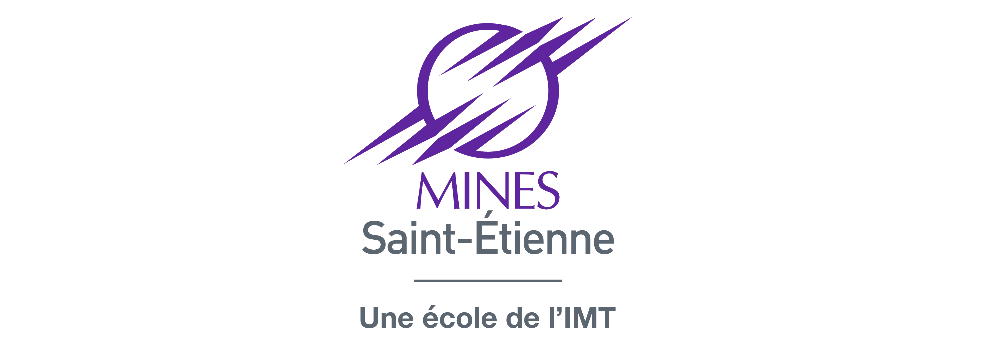
\includegraphics[scale=0.5]{Images/emse_new.png}
	\end{center}
	\end{figure}

\maketitle\thispagestyle{empty}
\newpage
\tableofcontents
\newpage

\section{Introduction}
L'Advenced Encryption Standard (ci-après AES) est, comme son nom l'indique, un standard de cryptage symétrique remplaçant le Data Encryption Standard (DES) qui était devenu inefficace notamment face aux attaques par force brute. Il a été instigué par le National Institue of Standards and Technology (NIST) le 2 janvier 1997. L'algorithme Rijindael a été proposé comme norme AES en octobre 2000, puis publié par le NIST dans la norme FIPS PUB 197 le 26 novembre 2001. C'est un algorithme de chiffrement par blocs supportant différentes combinaisons de longueurs de clés et longueurs de blocs. 
\par On distingue trois versions d’AES : AES-128, AES-192 et AES-256.
L’algorithme opère sur des blocs de 128 bits qu’il transforme en blocs cryptés de 128 bits à l’aide d’une clé de 128 bits (AES-128), 192 bits (AES-A92) ou 256 bits (AES-256). Cela nécessite respectivement 10, 12 ou 14 tours (aussi appelés round).
Chaque tour, à l’exception du dernier, comporte les mêmes étapes subdivisées en 4 transformations :
	\begin{itemize}
		\item[-] \emph{SubBytes}
		\item[-] \emph{AddRoundKey}
		\item[-] \emph{ShiftRows}
		\item[-] \emph{MixColumns}
	\end{itemize}
Une fonction supplémentaire est nécessaire pour la génération des clés des rounds. Il s'agit de la fonction \emph{AddRoundKey}.

\par Le but de ce projet était d'implémenter, en langage VHDL, l'algorithme de déchiffrement AES-128. 
\section{Principe de l'algorithme de déchiffrement}
L'algorithme de déchiffrement est assez semblable à l'algorithme de chiffrement. Le message chiffré va subir plusieurs transformations par blocs au cours de plusieurs round (11 en tout), selon les transformations suivantes:
	\begin{itemize}
		\item[-] \emph{InvSubBytes}
		\item[-] \emph{InvAddRoundKey}
		\item[-] \emph{InvShiftRows}
		\item[-] \emph{InvMixColumns}
	\end{itemize}
Ces blocs font bien entendu, comme leur nom l'indique, les opérations inverses des différents blocs de chiffrement. Ces blocs seront décrit de manière détaillée dans la suite de ce rapport. 
\newpage
De manière générale, on peut représenter le déchiffrement AES 128bits par l'algorigramme suivant:
	\begin{figure}[h]
	\begin{center}
	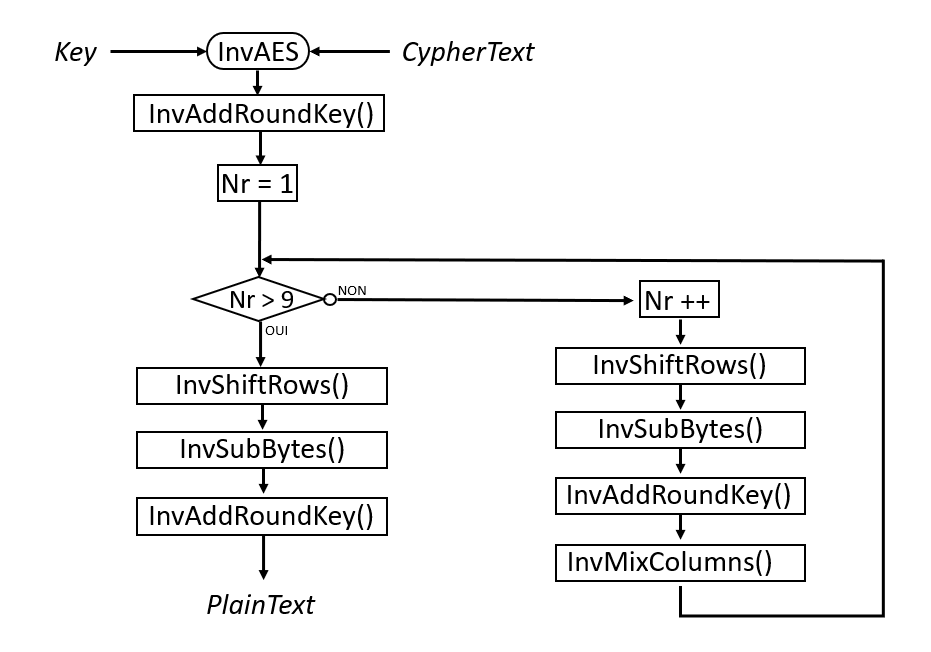
\includegraphics[scale=0.5]{Images/InvAESAlgorigramme.png}
	\end{center}
	\caption{Algorigramme de InvAES}
	\label{InvAES algorigramme}
	\end{figure}

Ce schéma peut se traduire par le pseudo-code suivant (fourni dans la FIPS 197): 
	\begin{figure}[H]
	\begin{center}
	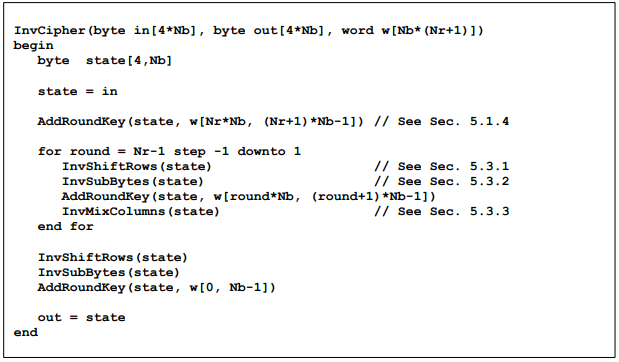
\includegraphics[scale=0.8]{Images/InvAESPseudoCode.png}
	\end{center}
	\caption{Pseudo-code de InvAES (FIPS 197)}
	\label{InvAES algorigramme}
	\end{figure}

\section{Implémentation des différents composants}
	Avant toute chose, il est important de noter qu'une librairie regroupant tous les différents types dont nous pourrions avoir besoin nous est fournie dans le fichier\\ \emph{state\_definition\_package.vhd}: 
	\begin{lstlisting}
	package state_definition_package is
  		subtype bit4 is std_logic_vector(3 downto 0);
  		subtype bit8 is std_logic_vector(7 downto 0);
 		subtype bit16 is std_logic_vector(15 downto 0);
  		subtype bit32 is std_logic_vector(31 downto 0);
 		subtype bit128 is std_logic_vector(127 downto 0);
  		type row_state is array(0 to 3) of bit8;
  		type column_state is array(0 to 3) of bit8;
  		type type_state is array(0 to 3) of row_state;
  		type type_shift is array(0 to 3) of integer range 0 to 3;
  		type type_temp is array(0 to 3) of bit8;
  		type row_key is array(0 to 3) of bit8;
  		type type_key is array(0 to 3) of row_key;
  		type reg_w is array(0 to 3) of bit32;
  		type type_rcon is array(0 to 10) of bit8;
  		constant Rcon : type_rcon := (X"01", X"02", X"04", X"08",
  		 X"10", X"20", X"40", X"80", X"1b", X"36", X"00");	
  		function "xor" ( L,R: column_state ) return column_state; 
	end state_definition_package;
	\end{lstlisting}
	Par exemple, \emph{bit8} représente un octet, \emph{column\_state} une colonne de 4 octets, \emph{type\_state} une matrice 4x4 d'octets, etc. Certains de ces types ont été utilisés lors de l'implémentation, et seront utilisés dans la suite de ce rapport.
	
Tous les tests ont été réalisés à partir des décompositions des étapes de déchiffrement du message original, fournies en fin de sujet du projet. Il faut faire attention au type des données. En effet, dans le sujet les valeurs sont données colonnes par colonnes (4 octets de la première colonne, puis 4 octets de la deuxième colonne, etc), alors que \emph{type\_state} est un tableau de ligne (cette confusion au niveau des données à traiter m'a fait perdre beaucoup de temps).

	\subsection{InvSBox}
		\subsubsection{Principe}
		L'algorithme AES utilise une table de substitution, appelée S-Box, dans la fonction \emph{InvSubBytes}. Cette table prend en entrée un octet, et fournie en sortie un autre octet. La figure suivante montre la S-Box inversée utilisée pour ce projet:
		\begin{figure}[H]
			\begin{center}
			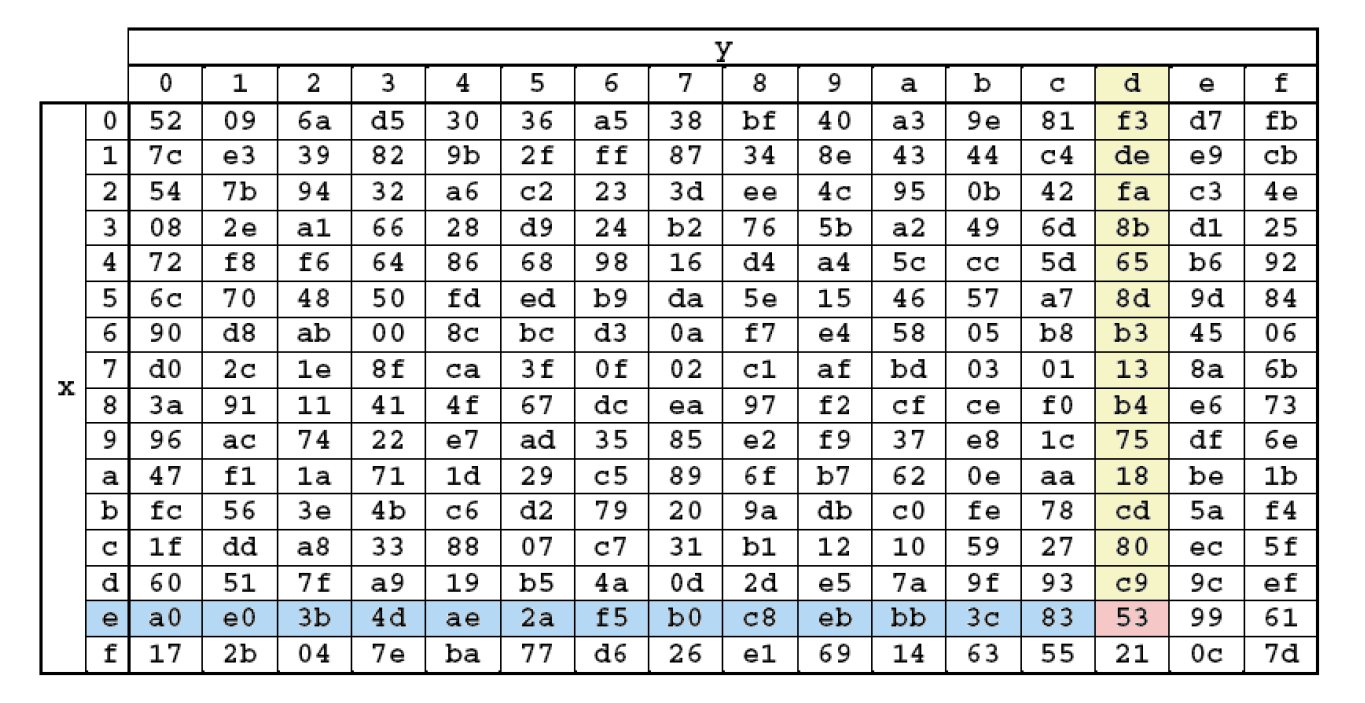
\includegraphics[scale=0.4]{Images/InvSBox.png}
			\end{center}
			\caption{Inverse de la S-Box}
			\label{InvSBox}
		\end{figure}
Par exemple, en entrant l'octet \emph{0xed}, on doit obtenir en sortie \emph{0x53}.
		\subsubsection{Implémentation}
	L'inverse de la S-Box a été implémenté sous forme d'un tableau de 256 cases de \emph{bit8} initialisé à la main. On peut représenter l'entité \emph{InvSBox} par le schéma suivant:
		\begin{figure}[H]
			\begin{center}
			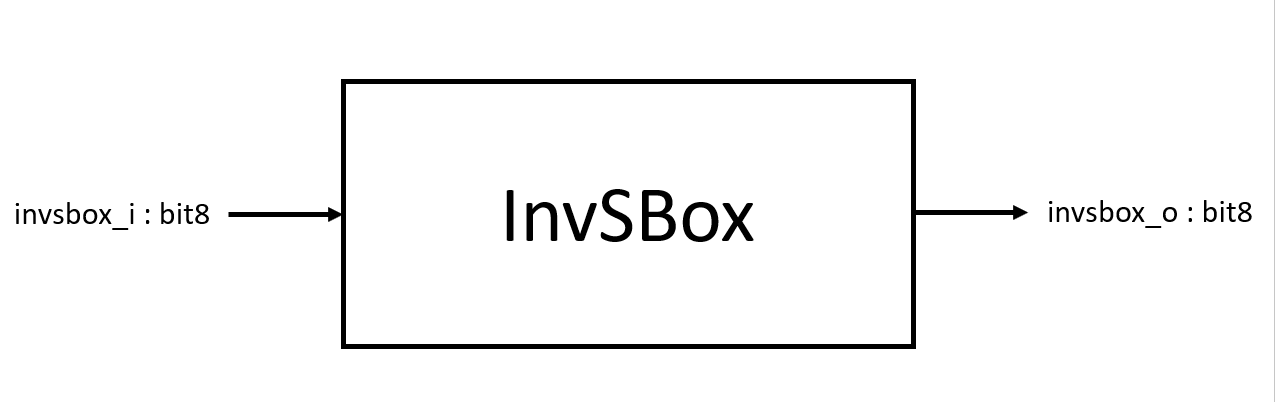
\includegraphics[scale=0.3]{Images/InvSBoxEntity.png}
			\end{center}
			\caption{Schéma de l'entité InvSBox}
			\label{InvSBoxEntity}
		\end{figure}
	L'implémentation de cette entité se trouve dans le fichier \emph{InvSBox.vhd}.
		
		\subsubsection{Tests et résultats}
	Le test bench \emph{InvSBox\_tb.vhd} a pour objectif de tester cette S-Box inversée. Plutôt que de tester quelques valeurs au hasard, il a été choisit de créer un processus dans lequel une variable s'incrémente toutes les 200 ns jusqu'à atteindre 255. (Une fois cette valeur atteinte, on remet la variable à 0 et on recommence l'incrémentation). On obtient alors le résultat suivant sur modelsim:
		\begin{figure}[H]
			\begin{center}
			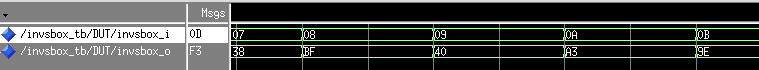
\includegraphics[scale=0.8]{Images/InvSBoxTb.png}
			\end{center}
			\caption{Résultat du test bench pour InvSBox}
			\label{InvSBoxTb}
		\end{figure}
	En se référant à la figure \ref{InvSBox}, page \pageref{InvSBox}, on constate que l'on obtient bien le bon résultat.
	
	\subsection{invSubBytes}
		\subsubsection{Principe}
	La fonction \emph{InvSubBytes} est une transformation non linéaire qui s'applique à tous les octets de l'état en utilisant la S-Box inversée obtenue précédemment. 	
		\subsubsection{Implémentation}
	Cette fonction prend donc en entrée une matrice 4x4 d'octet et retourne également une matrice 4x4 d'octet en ayant utilisée la S-Box inversée. On peut le représenter selon le schéma suivant:
		\begin{figure}[H]
			\begin{center}
			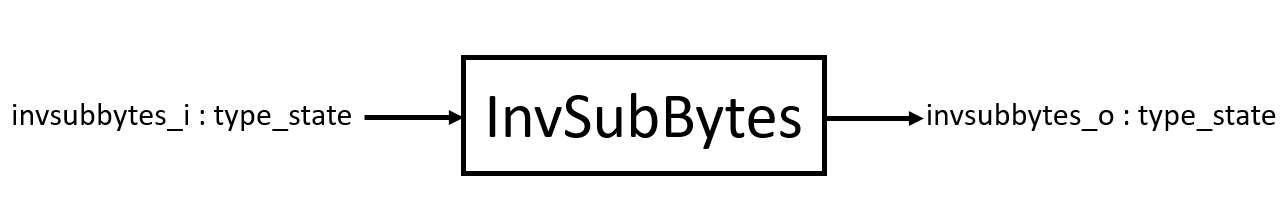
\includegraphics[scale=0.4]{Images/InvSubBytesEntity.png}
			\end{center}
			\caption{Schéma de l'entité InvSubBytes}
			\label{InvSubBytesEntity}
		\end{figure}
	Pour implémenter cela, on génère une matrice 4x4 de \emph{InvSBox} (une par octet). Ensuite, il s'agit simplement d'aller chercher la bonne valeur en fonction des coordonnées.
	
	L'implémentation de cette entité se trouve dans le fichier \emph{InvSubBytes.vhd}.
		\subsubsection{Tests et résultats}
		Pour tester cette partie, la matrice suivante a été entrée dans le test bench (matrice fournie à la fin du sujet pour le round 9 de la partie déchiffrement): \\
			\begin{table}[H]
				\begin{center}
				\begin{tabular}{|c|c|c|c|}
					\hline
					0x06 & 0x85 & 0xa6 & 0x61 \\
					\hline
					0x09 & 0xfb & 0x06 & 0x54 \\
					\hline
					0x99 & 0xc1 & 0x5f & 0xca \\
					\hline
					0x5b & 0x8e & 0x56 & 0x74 \\
					\hline
				\end{tabular}
				\caption{Matrice d'entrée du bloc InvSubBytes}
				\label{MatriceEntreeInvSubBytes}
				\end{center}
			\end{table}
			
		La matrice suivante doit être obtenue en sortie: \\
			\begin{table}[H]
				\begin{center}
				\begin{tabular}{|c|c|c|c|}
					\hline
					0xa5 & 0x67 & 0xc5 & 0xd8 \\
					\hline
					0x40 & 0x63 & 0xa5 & 0xfd \\
					\hline
					0xf9 & 0xdd & 0x84 & 0x10 \\
					\hline
					0x57 & 0xe6 & 0xb9 & 0xca \\
					\hline
				\end{tabular}
				\caption{Matrice de sortie du bloc InvSubBytes}
				\label{MatriceSortieInvSubBytes}
				\end{center}
			\end{table}
		La modélisation sur modelsim donne le résultat suivant:
		\begin{figure}[H]
			\begin{center}
			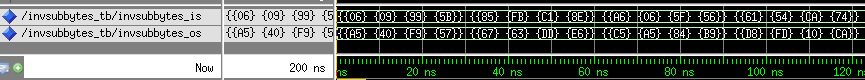
\includegraphics[scale=0.70]{Images/InvSubBytesTb.png}
			\end{center}
			\caption{Résultat du test bench pour InvSubBytes}
			\label{InvSubBytesTb}
		\end{figure}
	On constate alors que l'on obtient en sortie la matrice souhaitée. On peut donc valider le fonctionnement de cette partie.

	\subsection{InvAddRoundKey}
		\subsubsection{Principe}
	La fonction \emph{InvAddRoundKey} ajoute la clé de round courante à l'état (les clés de ronde sont obtenues à partir de la fonction \emph{KeyExpension} fournie, hormis pour la clé du round 0). Toutes ses clés sont directement accessibles depuis la librairie fournie avec le sujet. 
\par Elle est tout à fait semblable à la fonction \emph{AddRoundKey}. Cela implique donc qu'il s'agit simplement d'un XOR entre chaque octet de l'état et de la clé en question.
		\subsubsection{Implémentation}
	Cette fonction prend en entrée une matrice 4x4 d'octets et une matrice 4x4 correspondant à une clé. Elle fournie en sortie une matrice 4x4 d'octets, résultat du XOR entre l'état et la clé.
			\begin{figure}[H]
				\begin{center}
				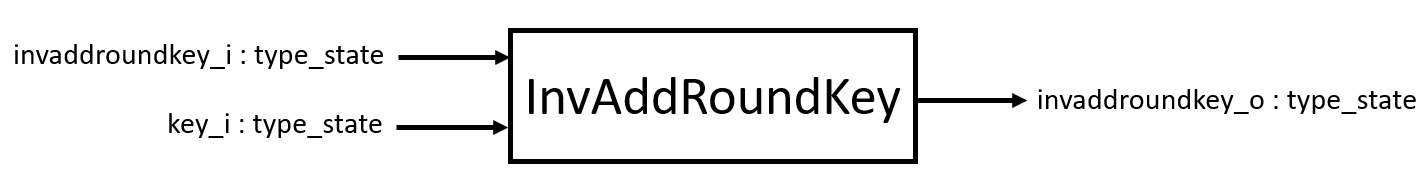
\includegraphics[scale=0.4]{Images/InvAddRoundKeyEntity.png}
				\end{center}
				\caption{Schéma de l'entité InvAddRoundKey}
				\label{InvAddRoundKeyEntity}
			\end{figure}
	L'implémentation de cette entité se trouve dans le fichier \emph{InvAddRoundKey.vhd}.
		\subsubsection{Tests et résultats}
		Pour tester cette partie, la matrice du message chiffré a été utilisée dans le test bench: \\
			\begin{table}[H]
				\begin{center}
				\begin{tabular}{|c|c|c|c|}
					\hline
					0xd6 & 0x4c & 0x47 & 0xd7 \\
					\hline
					0xef & 0xe8 & 0x6b & 0x6a \\
					\hline
					0xa6 & 0xef & 0x95 & 0xcd \\
					\hline
					0xdc & 0xd2 & 0x46 & 0xf0 \\
					\hline
				\end{tabular}
				\caption{Matrice d'entrée (message chiffré)du bloc AddRoundKey}
				\label{MatriceMessageInvAddRoundKey}
				\end{center}
			\end{table}
			
		Et la clé correspondante suivante a été utilisée:
		\begin{table}[H]
				\begin{center}
				\begin{tabular}{|c|c|c|c|}
					\hline
					0xd0 & 0xc9 & 0xe1 & 0xb6 \\
					\hline
					0x14 & 0xee & 0x3f & 0x63 \\
					\hline
					0xf9 & 0x25 & 0x0c & 0x0c \\
					\hline
					0xa8 & 0x89 & 0xc8 & 0xa6 \\
					\hline
				\end{tabular}
				\caption{Clé utilisée pour le round 10}
				\label{MatriceCleInvAddRoundKey}
				\end{center}
			\end{table}
			
		La matrice suivante doit alors être obtenue en sortie: \\
			\begin{table}[H]
				\begin{center}
				\begin{tabular}{|c|c|c|c|}
					\hline
					0x06 & 0x85 & 0xa6 & 0x61 \\
					\hline
					0xfb & 0x06 & 0x54 & 0x09 \\
					\hline
					0x5f & 0xca & 0x99 & 0xc1 \\
					\hline
					0x74 & 0x5b & 0x8e & 0x56 \\
					\hline
				\end{tabular}
				\caption{Matrice de sortie du bloc AddRoundKey}
				\label{MatriceSortieInvAddRoundKey}
				\end{center}
			\end{table}
			
La modélisation sur modelsim donne le résultat suivant:
		\begin{figure}[H]
			\begin{center}
			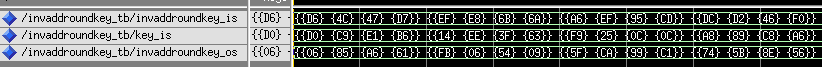
\includegraphics[scale=0.72]{Images/InvAddRoundKeyTb.png}
			\end{center}
			\caption{Résultat du test bench pour InvAddRoundKey}
			\label{InvAddRoundKeyTb}
		\end{figure}
	On constate alors que l'on retrouve en sortie la matrice souhaitée. On peut donc également valider le fonctionnement de cette partie.
	\subsection{InvShiftRows}
		\subsubsection{Principe}
	La fonction \emph{InvShiftRows} effectue une permutation cyclique des octets des lignes de l'état selon le schéma suivant: 
			\begin{figure}[H]
				\begin{center}
				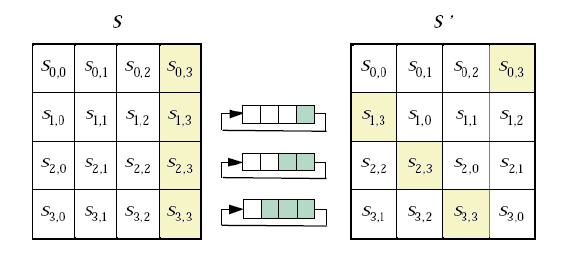
\includegraphics[scale=0.9]{Images/InvShiftRows.png}
				\end{center}
				\caption{Principe du InvShiftRows}
				\label{InvShiftRows}
			\end{figure}
	La rotation va dépendre de la ligne. Par exemple, pour la ligne 0 on fait une rotation de 0 octets (donc pas de rotations). Pour la ligne 1 on fera la rotation d'un octet: le dernier octet de la ligne passe en première position et les autres se retrouvent alors décalés de 1. Pour la deuxième ligne le dernier octet passe en deuxième position et l'avant dernier en première position. Les autres octets se retrouvent alors décalés de 2, et ainsi de suite. 
	
		\subsubsection{Implémentation}
	Cette fonction prend en entrée une matrice 4x4 d'octets et fournie en sortie une matrice 4x4.
			\begin{figure}[H]
				\begin{center}
				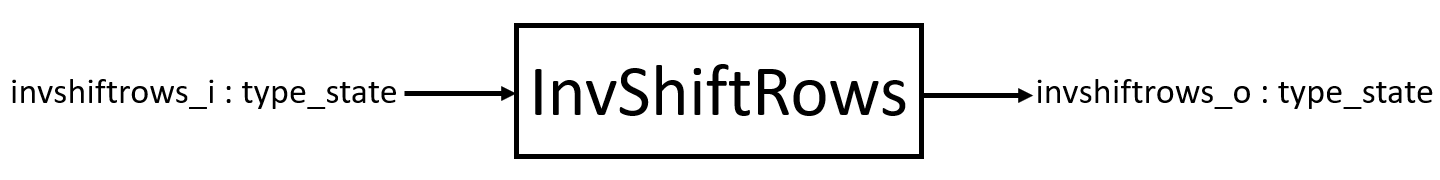
\includegraphics[scale=0.4]{Images/InvShiftRowsEntity.png}
				\end{center}
				\caption{Schéma de l'entité InvShiftRows}
				\label{InvShiftRowsEntity}
			\end{figure}
	L'implémentation de cette entité se trouve dans le fichier \emph{InvShiftRows.vhd}.			
			
		\subsubsection{Tests et résultats}
	Pour tester cette fonction, la matrice suivante a été passée en entrée (résultat de \emph{AddRoundKey} sur le message chiffré):
			\begin{table}[H]
				\begin{center}
				\begin{tabular}{|c|c|c|c|}
					\hline
					0x06 & 0x85 & 0xa6 & 0x61 \\
					\hline
					0xfb & 0x06 & 0x54 & 0x09 \\
					\hline
					0x5f & 0xca & 0x99 & 0xc1 \\
					\hline
					0x74 & 0x5b & 0x8e & 0x56 \\
					\hline
				\end{tabular}
				\caption{Matrice d'entrée du bloc InvShiftRows}
				\label{MatriceEntreeInvShiftRows}
				\end{center}
			\end{table}
			
			Normalement, la matrice suivante doit être obtenue en sortie:
			\begin{table}[H]
				\begin{center}
				\begin{tabular}{|c|c|c|c|}
					\hline
					0x06 & 0x85 & 0xa6 & 0x61 \\
					\hline
					0x09 & 0xfb & 0x06 & 0x54 \\
					\hline
					0x99 & 0xc1 & 0x5f & 0xca \\
					\hline
					0x5b & 0x8e & 0x56 & 0x74 \\
					\hline
				\end{tabular}
				\caption{Matrice de sortie du bloc InvShiftRows}
				\label{MatriceSortieInvShiftRows}
				\end{center}
			\end{table}
	La simulation sur modelsim nous donne le résultat suivant:
		\begin{figure}[H]
			\begin{center}
			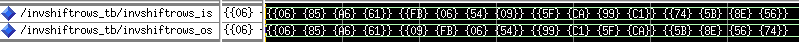
\includegraphics[scale=0.74]{Images/InvShiftRowsTb.png}
			\end{center}
			\caption{Résultat du test bench pour InvShiftRows}
			\label{InvShiftRowsTb}
		\end{figure}

	\subsection{InvMixColumns}
		\subsubsection{Principe}
La transformation \emph{InvMixColumns} s'applique colonne par colonne. Chaque octet de chaque colonne est multiplié par 9, 11, 13 et 14. La figure suivante illustre cette transformation:
		\begin{figure}[H]
			\begin{center}
			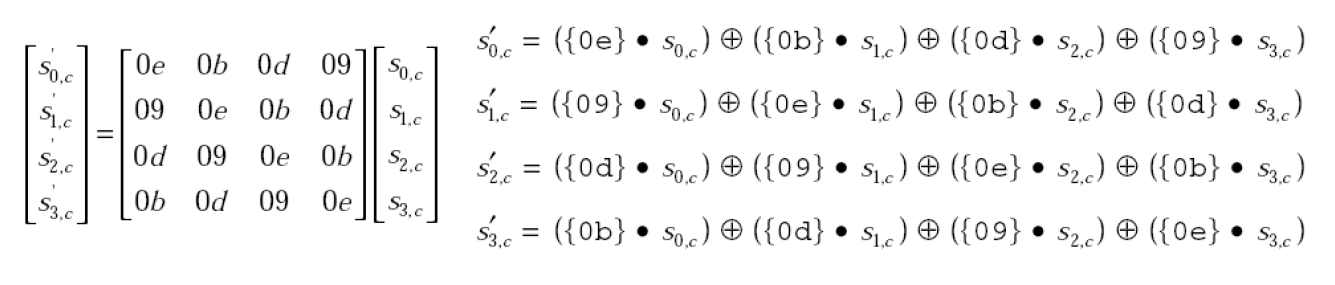
\includegraphics[scale=0.4]{Images/PrincipeInvMixColumns.png}
			\end{center}
			\caption{Illustration de la transformation opérée par InvMixColumn}
			\label{PrincipeInvMixColumns}
		\end{figure}
Toutes ces opérations se passent dans le corps de Galois. Les additions peuvent donc se calculer à l'aide d'un XOR. De manière générale, on peut décomposer une multiplication par 13 de la manière suivante:
		\begin{align*}
		13 \times x &= x \times (8 \oplus 4 \oplus 1) \\
					&= x \times (2^3 \oplus 2^2 \oplus 2^0) \\
					&= x \times ((2 \oplus 2 \oplus 2 \oplus 2) \oplus (2 \oplus 2) \oplus 1)
		\end{align*}
\par On remarque donc qu'au final, il ne s'agit que de multiplication et addition par 2 (plus éventuellement une addition avec l'élément lui-même), ce qui est finalement assez simple à mettre en place d'un point de vue informatique.
		
		\subsubsection{Implémentation}
	Etant donné que l'opération \emph{InvMixColumns} opère colonne par colonne, un bloc \emph{InvMixOneColumn} a été mis en place. Le bloc général \emph{InvMixColumns} fera alors appel 4 fois à cette plus petite entité.	L'entité \emph{InvMixOneColumn} prend donc en entrée une colonne de 4 octets, et donne le même type en sortie.
			\begin{figure}[H]
				\begin{center}
				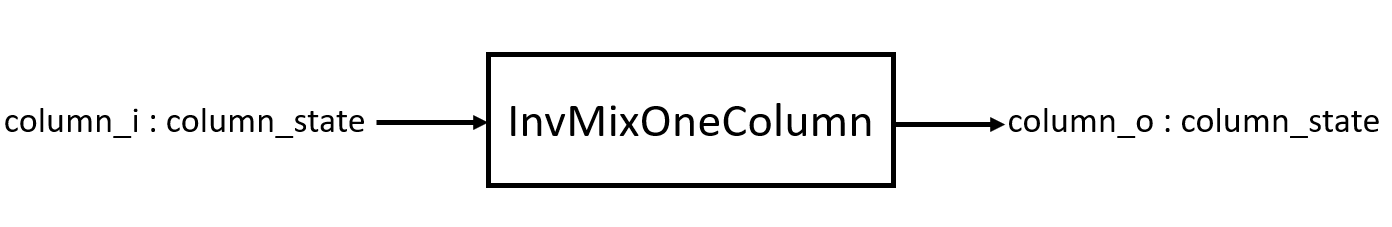
\includegraphics[scale=0.4]{Images/InvMixOneColumnEntity.png}
				\end{center}
				\caption{Schéma de l'entité InvMixOneColumn}
				\label{InvMixOneColumnEntity}
			\end{figure}
Pour implémenter cette transformation, des signaux intermédiaires de type \emph{column\_state} ont été créés afin de stocker les résultats des multiplications par 2, 4, 8, 9, 11, 13 et 14. En effet, chacun des résultats de ces multiplications utilise le résultat des multiplications précédentes. 
\par Pour multiplier par 2, il suffit de faire un décalage à gauche des bits et de compléter à droite avec un zéro. Si le bit de poids fort vaut 0, cela ne pose aucun problème, on reste sur 8 bits (le MSB n'a alors aucune importance). Cependant, si le bit de poids fort vaut 1, cela pose problème car on se retrouve alors sur 9 bits. Pour palier à ce problème, il suffit de faire un ou-exclusif avec la valeur b00011011. Ce ou-exclusif ne doit être appliqué que si le MSB initial vaut 1. Cependant, pour éviter de tester à chaque fois cette condition, on effectue systématiquement ce ou-exclusif, mais conditionné par le MSB de l'octet en question. En effet, si ce MSB vaut 0, alors le XOR n'a aucun effet. La ligne suivante illustre ce principe en VHDL:
		\begin{lstlisting}
	times2_s(i) <= (x_i(i)(6 downto 0)&'0') xor 
		("000"&x_i(i)(7)&x_i(i)(7)&'0'&x_i(i)(7)&x_i(i)(7));
		\end{lstlisting}
\par Une fois les multiplications par 8, 4 et 2 obtenues, il ne reste plus qu'à faire des XOR entre ces différents résultats pour obtenir les multiplications par 9, 11, 13 et 14.
Une fois tous ces résultats obtenus, il ne reste plus qu'à appliquer des XOR pour obtenir le résultat final, en suivant les opérations indiqués en figure \ref{PrincipeInvMixColumns} page \pageref{PrincipeInvMixColumns}.
\par Une fois que cette partie est fonctionnelle, il ne reste plus qu'à faire le bloc général \emph{InvMixColumns}. Celui-ci prend en entrée une matrice (de type\_state) et retourne également une matrice. 
			\begin{figure}[H]
				\begin{center}
				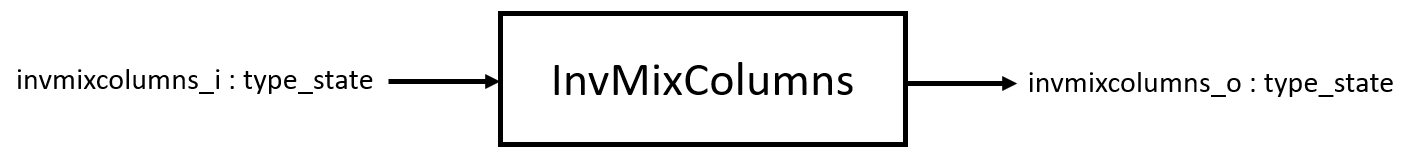
\includegraphics[scale=0.4]{Images/InvMixColumnsEntity.png}
				\end{center}
				\caption{Schéma de l'entité InvMixColumns}
				\label{InvMixColumnsEntity}
			\end{figure}
\par Cette partie est relativement simple à mettre en œuvre car elle fait appel à 4 \emph{InvMixOneColumn} (une pour chaque colonne). Le seul point particulier est le type de données traitées. En effet, \emph{InvMixOneColumn} travail sur des colonnes tandis que le type \emph{type\_state} est un tableau de ligne. Il faut donc créer des signaux intermédiaires pour récupérer des colonnes, puis de faire l'opération inverse une fois chaque colonne traitée. 

	L'implémentation de ces entités se trouve dans les fichiers \emph{InvMixColumns.vhd} et \emph{InvMixOneColumn}.
		
		\subsubsection{Tests et résultats}
Un premier test bench a été réalisé pour vérifier le fonctionnement de l'entité \emph{MixOneColumn}. Les résultats de ces tests ne sont pas développés ici, seul les résultats pour l'entité \emph{InvMixColumns} seront présentés (le bon fonctionnement de cette entité témoigne du bon fonctionnement de la sous entité). Pour tester \emph{InvMixColumns}, la matrice suivante a été utilisée en entrée (il s'agit de la matrice de sortie de \emph{AddRoundKey} du round 10):
			\begin{table}[H]
				\begin{center}
				\begin{tabular}{|c|c|c|c|}
					\hline
					0x09 & 0x7e & 0xed & 0x8f \\
					\hline
					0x37 & 0x99 & 0x74 & 0xa1 \\
					\hline
					0x9f & 0x01 & 0xad & 0x10 \\
					\hline
					0xa4 & 0xc7 & 0xf8 & 0xa4 \\
					\hline
				\end{tabular}
				\caption{Matrice d'entrée du bloc InvMixColumns}
				\label{MatriceEntreeInvMixColumns}
				\end{center}
			\end{table}
			Normalement, la matrice suivante doit être obtenue en sortie:
			\begin{table}[H]
				\begin{center}
				\begin{tabular}{|c|c|c|c|}
					\hline
					0x36 & 0x7e & 0x29 & 0xbf \\
					\hline
					0x2b & 0xe3 & 0x2d & 0xea \\
					\hline
					0xaa & 0x43 & 0xea & 0x0f \\
					\hline
					0xb2 & 0xff & 0x22 & 0xc0 \\
					\hline
				\end{tabular}
				\caption{Matrice de sortie du bloc InvMixColumns}
				\label{MatriceSortieInvMixColumns}
				\end{center}
			\end{table}
Voici les résultats obtenus en simulation:
			\begin{figure}[H]
				\begin{center}
				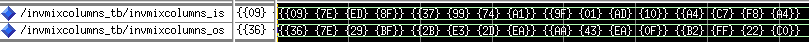
\includegraphics[scale=0.72]{Images/InvMixColumnsTb.png}
				\end{center}
				\caption{Résultat du test bench pour InvMixColumns}
				\label{InvMixColumnssTb}
			\end{figure}
On obtient bien le résultat escompté. 

	\subsection{Machine d'état}
		\subsubsection{Principe}
		Afin de pouvoir faire fonctionner l'algorithme de déchiffrement, une machine d'état (FSM) est nécessaire. Cette machine d'état va contrôler les différents états de l'algorithme et autoriser certaines sorties en fonction de ses états.
		\subsubsection{Implémentation}
		Pour implémenter cette FSM, l'architecture retenue est l'architecture de Moore. Ainsi, les sorties dépendent de l'état présent (synchrones, elles changent sur un front d'horloge), et l'état futur dépend de l'état présent et des entrées. 
Voici le schéma de cette entité:
			\begin{figure}[H]
				\begin{center}
				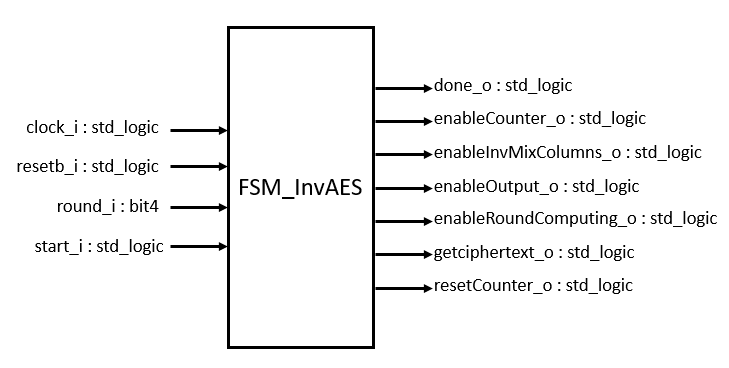
\includegraphics[scale=0.6]{Images/FSMInvAESEntity.png}
				\end{center}
				\caption{Schéma de l'entité FSM\_InvAES}
				\label{FSMInvAESEntity}
			\end{figure}
\par Voici la signification des entrées et sorties:
			\begin{itemize}
				\item[-] \emph{clock\_i} représente l'horloge
				\item[-] \emph{resetb\_i} permet d'initialiser le circuit (reset à l'état bas)
				\item[-] \emph{round\_i} désigne le numéro du round actuel
				\item[-] \emph{start\_i} permet de débuter le calcul
				\item[-] \emph{done\_o} indique la fin du calcul
				\item[-] \emph{enableCounter\_o} autorise la décrémentation du compteur
				\item[-] \emph{enableMixColumns\_o} autorise l'étape \emph{InvMixColumns}
				\item[-] \emph{enableOutput\_o} autorise la sortie
				\item[-] \emph{enableRoundComputing\_o} autorise l'étape \emph{InvSubBytes} et \emph{InvShiftRows}
				\item[-] \emph{getciphertext\_o} permet de récupérer le texte chiffré
				\item[-] \emph{resetCounter\_o} permet de réinitialiser le décompteur	\\
			\end{itemize} 
\par Pour implémenter cette partie, le graph d'état suivant a été retenu:
			\begin{figure}[H]
				\begin{center}
				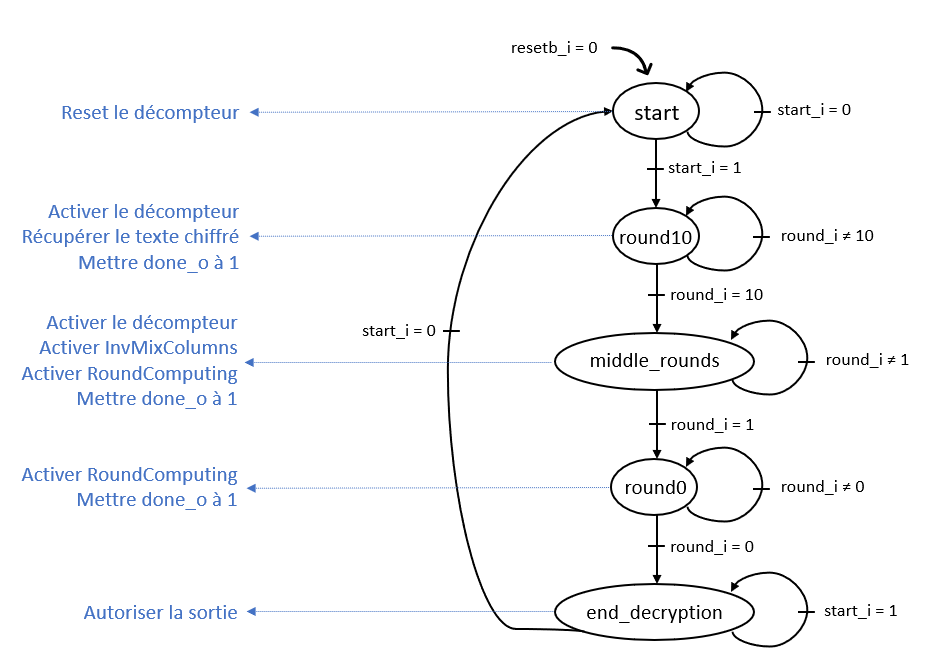
\includegraphics[scale=0.6]{Images/FSMInvAES.png}
				\end{center}
				\caption{Graph d'état pour Inv\_AES}
				\label{FSMInvAES}
			\end{figure}
	Sur ce graph, la sortie \emph{done\_o} est mise à 1 lorsque le calcul est en cours et non lorsqu'il est fini, car sur le schéma général le signal \emph{done\o} correspond au signal \emph{aes\_on\_o} qui indique que le calcul est en cours. Une autre solution aurait été d'ajouter dans l'entité générale un inverseur sur ce signal, comme cela est fait pour le signal \emph{reset\_i}.
		L'implémentation de cette entité se trouve dans le fichier \emph{FSM\_InvAES.vhd}.

		\subsubsection{Tests et résultats}
	Pour tester cette partie, les signaux suivants ont été utilisés dans le test bench (le décompteur a été décrémenté à la main):
		\begin{lstlisting}
resetb_is <= '1', '0' after 30 ns, '1' after 40 ns;
start_is <= '0', '1' after 50 ns, '0' after 200 ns;
clock_is <= not clock_is after 25 ns;
round_is <= "1010" after 100 ns, "1001" after 150 ns, "1000" after 200 ns, 
	"0111" after 250 ns, "0110" after 300 ns, "0101" after 350 ns, 
	"0100" after 400 ns, "0011" after 450 ns, "0010" after 500 ns, 
	"0001" after 550 ns, "0000" after 600 ns;
		\end{lstlisting}

On obtient le résultat suivant:
			\begin{figure}[H]
				\begin{center}
				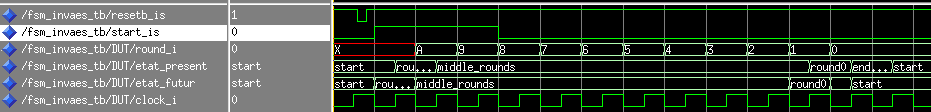
\includegraphics[scale=0.64]{Images/FSMInvAESTb.png}
				\end{center}
				\caption{Résultat du test bench pour FSM\_InvAES}
				\label{FSMInvAESTb}
			\end{figure}
On remarque que l'on obtient bien le fonctionnement attendu par le graph d'état. On peut donc valider le fonctionnement de cette partie. 
	\subsection{Décompteur}
		\subsubsection{Principe}
	Afin de pouvoir savoir dans quel round on se trouve, il est nécessaire d'implémenter un décompteur. Ce décompteur doit pouvoir être initialisé à une certaine valeur, et se décrémenter à chaque coup d'horloge. A noter également qu'il faudra gérer un éventuel débordement et empêcher au décompteur de se décrémenter lorsqu'il atteint 0.
		\subsubsection{Implémentation}
Ainsi, le décompteur dispose de 3 entrées (une horloge, un signal d'initialisation et un signal d'autorisation à se décrémenter) et une sortie correspondant aux différentes valeurs prises par cette entité.
			\begin{figure}[H]
				\begin{center}
				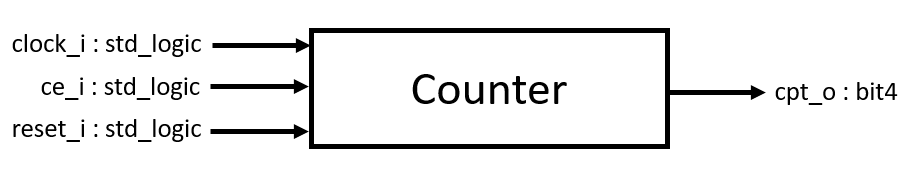
\includegraphics[scale=0.5]{Images/CounterEntity.png}
				\end{center}
				\caption{Schéma de l'entité Counter}
				\label{CounterEntity}
			\end{figure}
On peut remarquer que le reset du décompteur est un reset à l'état haut. En effet, dans la FSM la sortie \emph{resetCounter\_o} est mise à 1 lorsque nous voulons reset le counter (il est plus logique, de premier abord, de mettre à 1 une sortie que l'on veut activer). On pourrait également plutôt mettre un reset à l'état bas en modifiant seulement la valeur de \emph{resetCounter\_o} dans la FSM en fonction des états présents. Ici, le reset à l'état haut a été gardé.
	L'implémentation de cette entité se trouve dans le fichier \emph{Counter.vhd}.

		\subsubsection{Tests et résultats}
	Le test bench du décompteur nous permet d'obtenir le résultat suivant:
			\begin{figure}[H]
				\begin{center}
				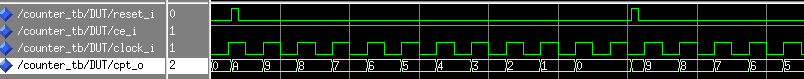
\includegraphics[scale=0.7]{Images/CounterTb.png}
				\end{center}
				\caption{Résultat du test bench pour l'entité Counter}
				\label{CounterTb}
			\end{figure}
Le décompteur prend donc toutes les valeurs de 10 à 0, ce qui permet bien de pouvoir accéder par la suite à tous les états de la FSM. On remarque aussi que le décompteur conserve bien la valeur 0 jusqu'à un nouveau reset. On peut donc valider le fonctionnement de cette entité.

	\subsection{Registre}
		\subsubsection{Principe}
	Un registre est nécessaire dans l'entité générale de InvAES afin de pouvoir sauvegarder en mémoire pendant un certains temps le résultat. Pour faire cela, on utilise un registre. Il s'agit en réalité d'une simple bascule D. Cette entité sera nommée \emph{RTL\_REG}. 
	
		\subsubsection{Implémentation}
Etant donné qu'il s'agit d'une bascule D, on retrouve en entrée une horloge, un reset (ici à l'état bas), un signal d'autorisation et l'entrée des données. Il y a une seule sortie, celle des données. On a donc l'entité suivante:
			\begin{figure}[H]
				\begin{center}
				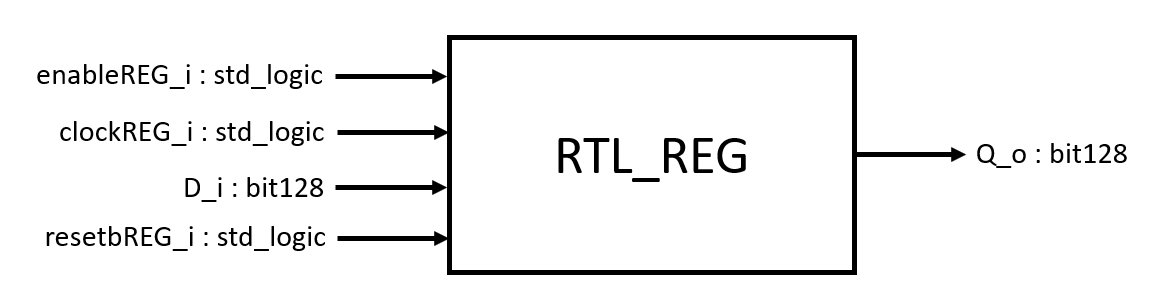
\includegraphics[scale=0.4]{Images/REGEntity.png}
				\end{center}
				\caption{Schéma de l'entité RTL\_REG}
				\label{REGEntity}
			\end{figure}
Ce registre est consitué de deux processus séquentiels. Le premier est utilisé pour le reset du registre et le second pour garder en mémoire ou non la donnée.
	L'implémentation de cette entité se trouve dans le fichier \emph{RTL\_REG.vhd}. 
		
		\subsubsection{Tests et résultats}
	Je n'ai pas réalisé de test bench pour cette entité car il s'agit d'une simple bascule D et une partie du cours a été donnée lors d'une séance de cours.

	\subsection{InvAESRound}
		\subsubsection{Principe}
Cette partie permet de réaliser toutes les étapes d'un round en fonction du round considéré. Ainsi, cette entité fait appel à \emph{InvSubBytes}, \emph{InvShiftRows}, \emph{InvMixColumns} et \emph{InvAddRoundKey}.
		\subsubsection{Implémentation}
Cette entité prend donc en entrée le signal \emph{enableInvMixColumns\_i}, le signal \emph{enableRoundComptuing\_i}, le signal \emph{resetb\_i}), le texte courant (\emph{currenttext\_i}), la clé du round correspondant (\emph{currentkey\_i}) et une horloge (\emph{clock\i}). En sortie, on retrouve un bit128.

Comme on ne fait pas toutes les étapes dans tous les rounds, il faut sélectionner quelles sous-entités sont utilisées en fonction du round. Pour cela, deux multiplexeurs sont utilisés. Pour cela, un composant à part a été crée (\emph{Multiplexer\_type\_state.vhd}). Ce multiplexer travail avec le type \emph{type\_state}.

De même, afin de pouvoir garder un minimum la valeur de sortie en mémoire, il faut un registre. Celui-ci a été implémenté directement à l'intérieur de l'entité \emph{InvAESRound} (les essais pour réutiliser le registre \emph{RTL\_REG} n'ont pas été très concluants) sous forme d'un processus combinatoire.

Enfin, les données d'entrée et de sortie sont du type \emph{bit128}. Cependant, les sous-entités utilisent le type \emph{type\_state}. Il faut donc faire une conversion de type (de bit128 à type\_state et inversement). Pour faire ces conversions, il faut appliquer le pseudo-code suivant: \\
{\fontfamily{lmtt}\selectfont 
	- - Conversion bit128 en type\_state \par
	k entier \par
	l entier \par
	Pour i allant de 0 à 3 faire \par
		\hspace*{1cm} Pour j allant de 0 à 3 faire \par
			\hspace*{2cm} k := 127-8*(i+j*4) \par
			\hspace*{2cm} l := 127-8*(i+j*4+1) \par
			\hspace*{2cm} MatriceTypeState[i][j] := TypeBit128[k à l] \par
		\hspace*{1cm} fin pour \par
	fin pour \\ \\
	
	- - Conversion type\_state en bit128 \par
	k entier \par
	l entier \par
	Pour i allant de 0 à 3 faire \par
		\hspace*{1cm} Pour j allant de 0 à 3 faire \par
			\hspace*{2cm} k := 127-8*(i+j*4) \par
			\hspace*{2cm} l := 127-8*(i+j*4+1) \par
			\hspace*{2cm} TypeBit128[k à l] := MatriceTypeState[i][j] \par
		\hspace*{1cm} fin pour \par
	fin pour \\
}
Je n'ai pas trouvé la formule de conversion seul. Un camarade (Cédric GERNIGON) me l'a donnée.

Au final, on dispose de l'entité suivante:
			\begin{figure}[H]
				\begin{center}
				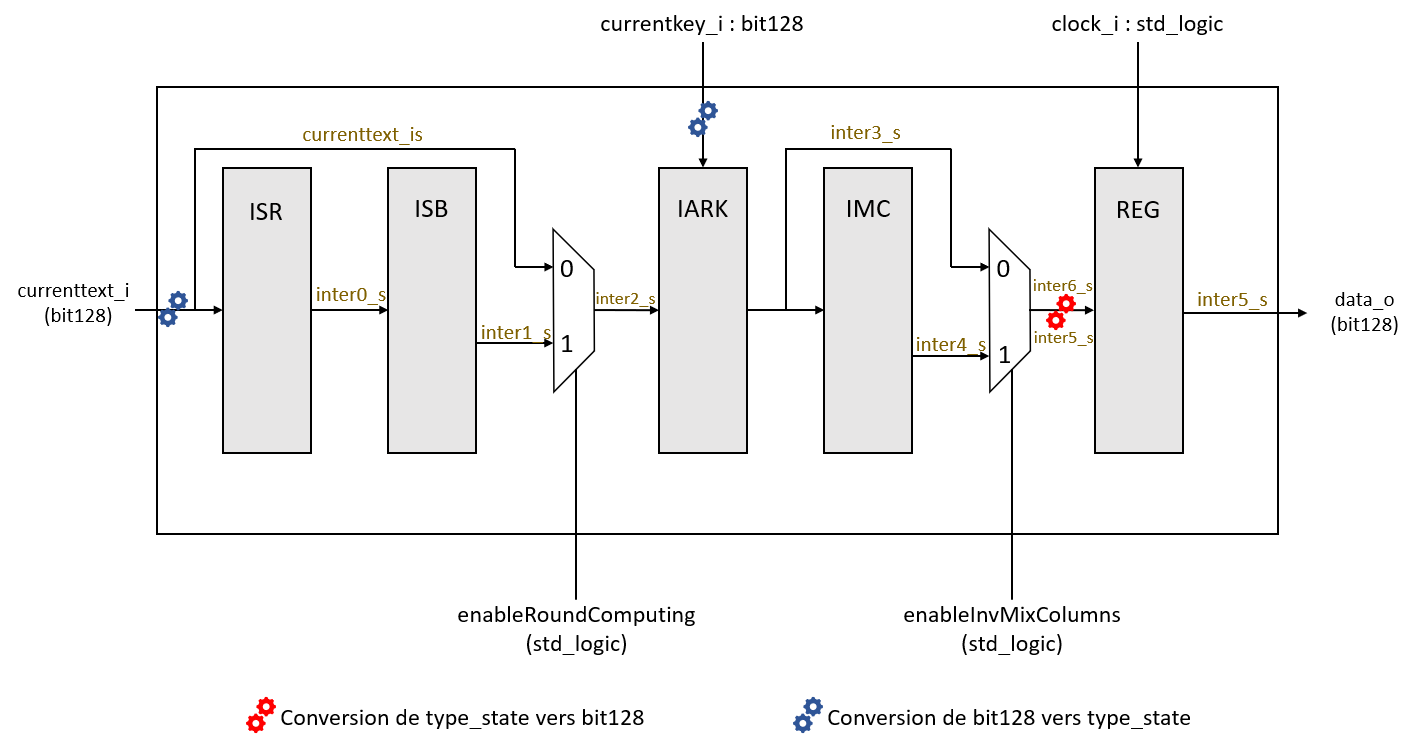
\includegraphics[scale=0.43]{Images/InvAESRoundEntity.png}
				\end{center}
				\caption{Schéma de l'entité InvAESRound}
				\label{InvAESRoundEntity}
			\end{figure}
			
La conversion de type aurait également pu se faire dans une entité à part entière.
	L'implémentation de l'entité \emph{InvAESRound} se trouve dans le fichier \emph{InvAESRound.vhd}.

		\subsubsection{Tests et résultats}
Cette entité à été testée pour le round 10 et 9. Seuls les résultats pour le round 10 sont détaillés ici. Ainsi, les matrices d'entrée sont les suivantes:
			\begin{table}[H]
				\begin{center}
				\begin{tabular}{|c|c|c|c|}
					\hline
					0xd6 & 0x4c & 0x47 & 0xd7 \\
					\hline
					0xef & 0xe8 & 0x6b & 0x6a \\
					\hline
					0xa6 & 0xef & 0x95 & 0xcd \\
					\hline
					0xdc & 0xd2 & 0x46 & 0xf0 \\
					\hline
				\end{tabular}
				\caption{\emph{currenttext\_i} pour le round 10}
				\label{CurrenttextRound10}
				\end{center}
			\end{table}
			
			\begin{table}[H]
				\begin{center}
				\begin{tabular}{|c|c|c|c|}
					\hline
					0xd0 & 0xc9 & 0xe1 & 0xb6 \\
					\hline
					0x14 & 0xee & 0x3f & 0x63 \\
					\hline
					0xf9 & 0x25 & 0x0c & 0x0c \\
					\hline
					0xa8 & 0x89 & 0xc8 & 0xa6 \\
					\hline
				\end{tabular}
				\caption{\emph{currentkey\_i} pour le round 10}
				\label{CurrentKeyRound10}
				\end{center}
			\end{table}
			
On doit normalement obtenir la matrice suivante en sortie:
			\begin{table}[H]
				\begin{center}
				\begin{tabular}{|c|c|c|c|}
					\hline
					0x06 & 0x85 & 0xa6 & 0x61 \\
					\hline
					0xfb & 0x06 & 0x54 & 0x09 \\
					\hline
					0x5f & 0xca & 0x99 & 0xc1 \\
					\hline
					0x74 & 0x5b & 0x8e & 0x56 \\
					\hline
				\end{tabular}
				\caption{Résultat de InvAESRound pour le round 10}
				\label{MatriceSortieInvAESRound}
				\end{center}
			\end{table}
			
Le test bench nous donne le résultat suivant:
			\begin{figure}[H]
				\begin{center}
				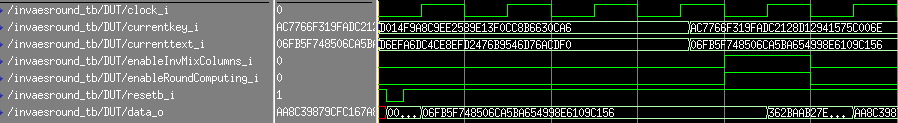
\includegraphics[scale=0.68]{Images/InvAESRoundTb.png}
				\end{center}
				\caption{Résultat du test bench pour l'entité InvAESRound}
				\label{InvAESRoundTb}
			\end{figure}
On obtient bien le résultat attendu. On remarque sur ce test bench le résultat sorti pour le round 9 (qui correspond lui aussi à ce que l'on doit obtenir) qui dure bien un cycle d'horloge.

		
\section{Implémentation globale de InvAES}
	\subsection{Principe}
Une fois tous ces composants crés, il ne reste plus qu'à les rassembler au sein de l'entité générale \emph{InvAES}. Il faut noter que le composant \emph{KeyExpansion\_table} est déjà fourni, c'est pourquoi il n'a pas été détaillé comme les autres composants. Il a seulement pour but de fournir la bonne clé intermédiaire en fonction du round. 
	\subsection{Implémentation}
	Pour implémenter cette entité générale, on utilise le schéma suivant:
			\begin{figure}[H]
				\begin{center}
				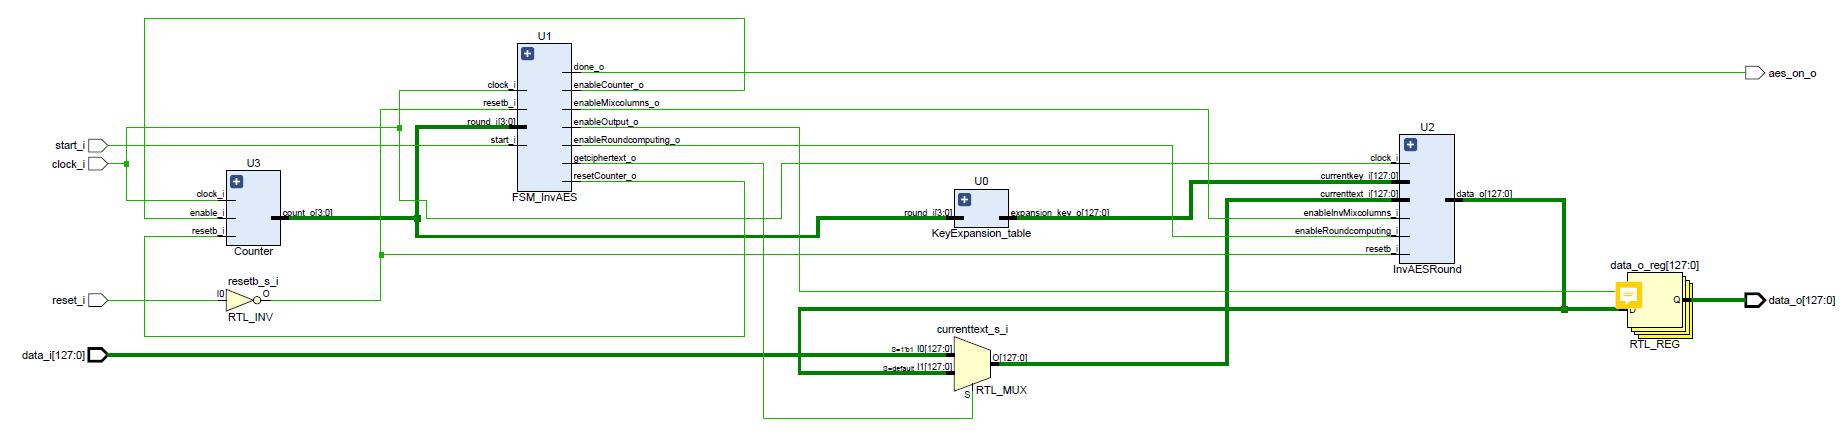
\includegraphics[scale=0.3]{Images/InvAESEntity.png}
				\end{center}
				\caption{Schéma de l'entité générale InvAES}
				\label{InvAESRoundEntity}
			\end{figure}
La première chose que l'on remarque est l'inverseur. En effet, le signal de reset passé en entrée est actif haut. Cependant, de nombreux composants internes utilisent un signal de reset actif bas. Cet inverseur a été simplement implémenté directement dans l'entité générale.

De plus, on peut également apercevoir un multiplexeur. Celui-ci à été implémenté directement, sous forme d'un processus séquentiel, dans l'entité générale plutôt que d'en faire une entité à part entière.
	L'implémentation de cette entité se trouve dans le fichier \emph{InvAES.vhd}.
	
	\subsection{Tests et résultats}
Pour tester le bon fonctionnement général, on envoie en entrée le texte chiffré et la clé correspondante. On doit retrouver en sortie le texte \emph{"Resto en ville ?"}. Voici le résultat obtenu sur modelsim:
			\begin{figure}[H]
				\begin{center}
				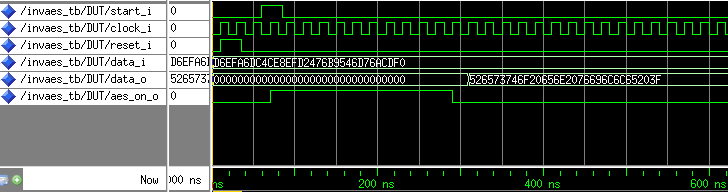
\includegraphics[scale=0.68]{Images/InvAESTb1.png}
				\end{center}
				\caption{Résultat du test bench pour l'entité InvAES}
				\label{InvAESRoundTb1}
			\end{figure}
			
Une fois le résultat affiché en ASCII on trouve:
			\begin{figure}[H]
				\begin{center}
				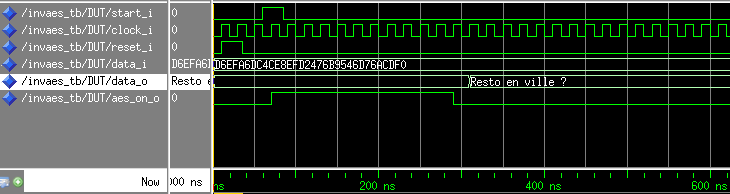
\includegraphics[scale=0.68]{Images/InvAESTb2.png}
				\end{center}
				\caption{Résultat du test bench pour l'entité InvAES affiché en ASCII}
				\label{InvAESRoundTb2}
			\end{figure}
On obtient le résultat attendu. On remarque bien que \emph{aes\_on\_o} est à 1 pendant 11 coups d'horloge.\\ On peut également noter que la simulation sur modelsim nous fait apparaître des warnings. Aucune solution n'a été trouvée pour résoudre ce problème, qui ne semble pas avoir d'importance pour le résultat final.
Néanmoins, notre déchiffrement AES fonctionne.

En regardant le résultat attendu dans le sujet, on remarque qu'il y a également un autre message que l'on peut passer au déchiffrement. Le sujet indique que ce message est la réponse d'Alice. ce message chiffré est: \par \begin{center}{\fontfamily{lmtt}\selectfont x"d7ca070cc0d3ce1e3943287756404506"} \end{center} \par On obtient alors le résultat suivant sur modelsim:
			\begin{figure}[H]
				\begin{center}
				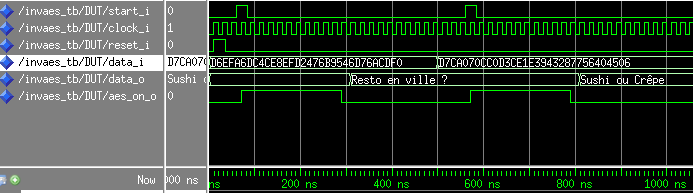
\includegraphics[scale=0.68]{Images/InvAESTb3.png}
				\end{center}
				\caption{Résultat final du déchiffrement}
				\label{InvAESRoundTb3}
			\end{figure}
On obtient donc ce qui semble être la réponse de Alice à Bob.

\section{Conclusion}
Ce projet m'a permit de comprendre l'intérêt et le principe du langage de description qu'est le VHDL. Les plus grosses difficultés se sont situées au début du projet et à la fin. En effet, au début je ne maitrisais pas assez bien le cours et ce langage de description pour pouvoir avancer assez rapidement. A ce moment, il m'a fallu beaucoup de temps pour bien assimiler les principes d'entités, d'architectures et de configurations. De plus, la plupart des erreurs étaient des erreurs de syntaxes. Une fois ces problèmes surmontés, la réalisation des différents composants a été assez simple une fois le principe de fonctionnement du composant compris. Enfin, j'ai du passer beaucoup de temps lors de la réalisation finale (pour \emph{InvAESRound} et \emph{InvAES}) pour que tout fonctionne. Il y avait de nombreux problèmes entre des signaux actifs à l'état bas ou haut, avec des \emph{reset} et \emph{init} activés au mauvais moment ou bien encore avec des \emph{start} dans les test bench qui ne duraient pas assez longtemps pour être actifs sur un front montant d'horloge (c'est ce type d'erreur qui m'a fait perdre le plus de temps à la fin).\\ Mais au final le déchiffrement fonctionne correctement.

\newpage

\newpage
\listoffigures
\listoftables


\end{document}